\documentclass[tikz]{standalone}

\usepackage{amsmath}
\usepackage{unicode-math}
\usepackage{mathtools}
\usepackage{derivative}

\setmainfont{Stix Two Text}
\setmathfont{Stix Two Math}

\usetikzlibrary{arrows.meta,fit,positioning}

\renewcommand{\familydefault}{\sfdefault}

% prefix equation numbers with section number
\numberwithin{equation}{section}

\DeclarePairedDelimiter{\ceil}{\lceil}{\rceil}
\DeclarePairedDelimiter{\floor}{\lfloor}{\rfloor}
\DeclarePairedDelimiter{\abs}{\lvert}{\rvert}
\DeclarePairedDelimiter{\norm}{\lVert}{\rVert}
\DeclarePairedDelimiter{\bra}{\langle}{\rvert}
\DeclarePairedDelimiter{\ket}{\lvert}{\rangle}
\DeclarePairedDelimiter{\expval}{\langle}{\rangle}
\DeclarePairedDelimiter{\norder}{\mathcolon}{\mathcolon}
\DeclarePairedDelimiter{\anorder}{\typecolon}{\typecolon}
	
\newcommand{\laplace}{\mbfnabla^2}
\newcommand{\trans}{{\scriptscriptstyle\mathsf{T}}}

\newcommand{\vdot}{\cdot}
\newcommand{\vcross}{\vectimes}
\newcommand{\vb}[1]{\symbfup{#1}}
\newcommand{\vu}[1]{\hat{\vb{#1}}}
\newcommand*\dd[2][\relax]{\mathop{\ifx\relax#1\odif{#2}\else \odif[order={#1}]{#2}\fi\,}}

\newcommand{\vacuum}{\ket*{\vb{0}}}

\DeclareMathOperator{\trace}{Tr}
\DeclareMathOperator{\sinc}{sinc}

\AtBeginDocument{
	\let\Re\relax
	\let\Im\relax
	\DeclareMathOperator{\Re}{Re}
	\DeclareMathOperator{\Im}{Im}

	\renewcommand{\div}{\mathop{\mbfnabla\vdot}}
	\newcommand{\curl}{\mathop{\mbfnabla\vectimes}}
}

\DeclarePairedDelimiterX{\comm}[2]{[}{]}{#1,#2}

\DeclarePairedDelimiterX{\braket}[2]{\langle}{\rangle}{#1\delimsize\vert#2}
\DeclarePairedDelimiterX{\ketbra}[1]{\lvert}{\rvert}{#1\rangle\delimsize\langle#1}



\begin{document}
	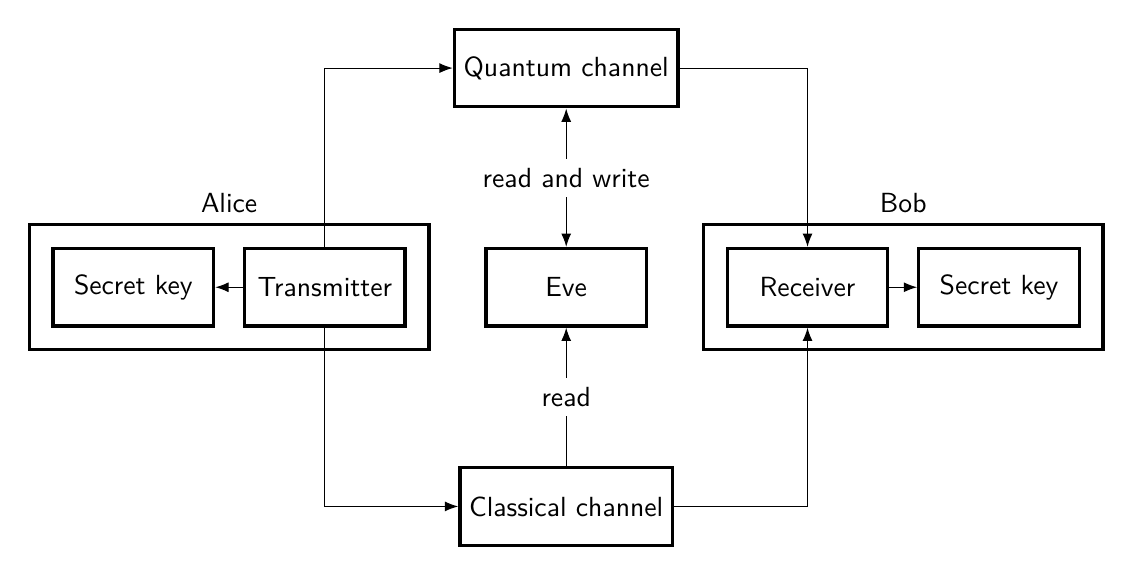
\begin{tikzpicture}[
		node distance=10pt,
		action/.style={midway, fill=white, align=center},
		block/.style={draw, very thick, fill=white, minimum height=28pt, minimum width=58pt},
		superblock/.style={draw, very thick, inner sep=8pt},
	]
		\node (ka) [block] {Secret key};
		\node (tx) [block, right=of ka] {Transmitter};
		\node [superblock, fit=(ka) (tx), label={Alice}] (alice) {};
		\node [block, right=28pt of tx] (eve) {Eve};
		\node (rx) [block, right=28pt of eve] {Receiver};
		\node (kb) [block, right=of rx] {Secret key};
		\node (bob) [superblock, fit=(rx) (kb), label={Bob}] {};
		
		\node (qch) [block, above=5em of eve] {Quantum channel};
		\node (cch) [block, below=5em of eve] {Classical channel};
		
		\draw[-Latex] (tx) -- (tx.north|-qch) -- (qch);
		\draw[-Latex] (qch) -- (qch-|rx.north) -- (rx);
		\draw[-Latex] (tx) -- (tx.south|-cch) -- (cch);
		\draw[-Latex] (cch) -- (cch-|rx.south) -- (rx);
		
		\draw[Latex-Latex] (eve) -- (qch) node[midway, fill=white] {read and write};
		\draw[Latex-] (eve) -- (cch) node[midway, fill=white]{read};
		
		\draw[-Latex] (tx) -- (ka);
		\draw[-Latex] (rx) -- (kb);
	\end{tikzpicture}
\end{document}
